\section{Section 2}

One can identify the top and bottom ten services based on total number of 
applications received for 2022 to 2023. Note that the bottom 10 services 
have zero number of applications received. This is not an exhasted list 
since there are other services that also have zero application. 

\begin{figure}
    \centering
    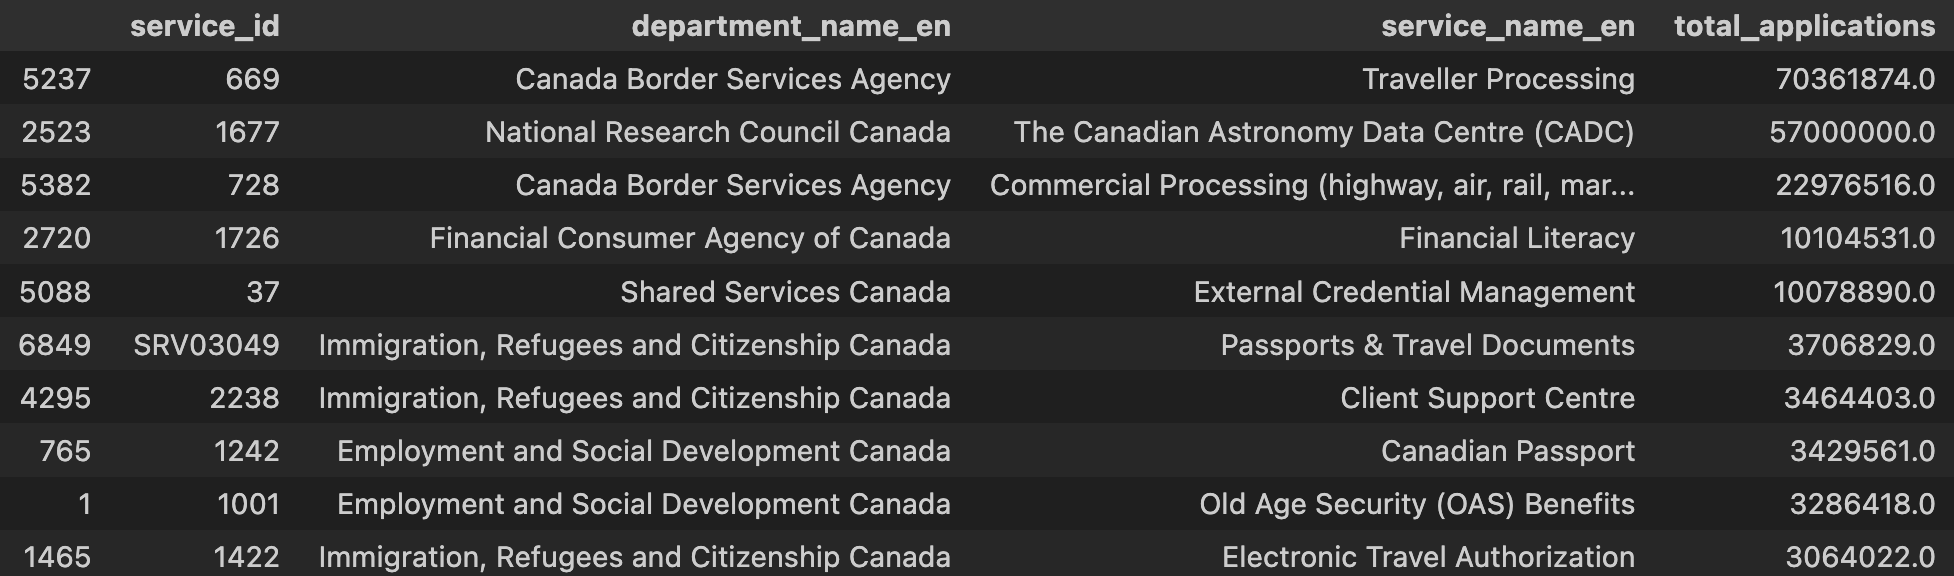
\includegraphics[width=1\linewidth]{Top10Svc.png}
    \caption{\label{fig:Top10}Top 10 Services by Application Volume}
\end{figure}

\begin{figure}
    \centering
    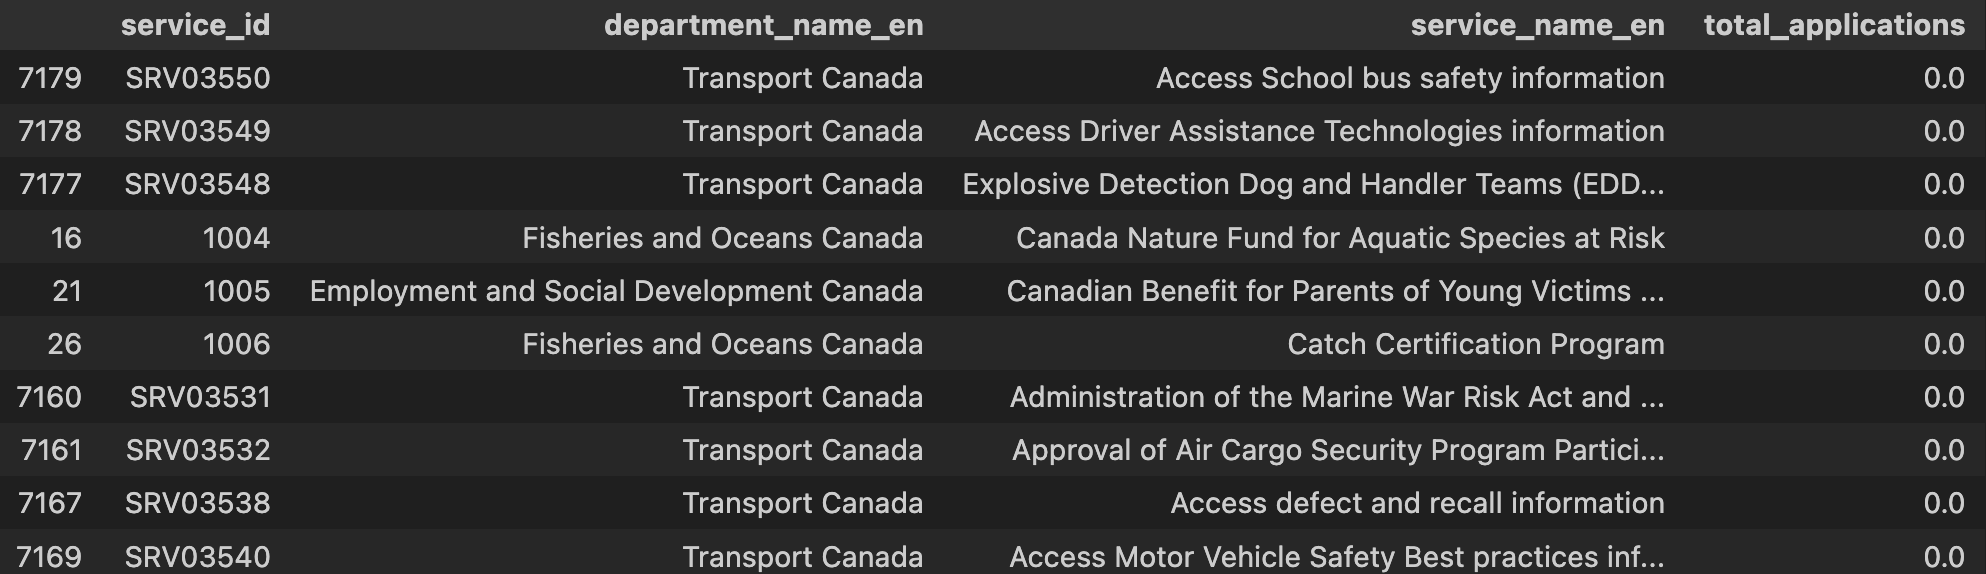
\includegraphics[width=1\linewidth]{Bottom10Svc.png}
    \caption{\label{fig:Bottom10}Bottom 10 Services by Application Volume}
\end{figure}

Services can be provided online to Canadians from end to end. There are 
six types of task: client can register for a personal account, can 
authenticate their identity, can apply for a service, can be notified of 
the outcome of their request, can receive the service and can provide 
feedback. Due to the limit that the author of this report doesn't have 
information on the definition of end-to-end, one should assume that 
services can be done online end-to-end only if all six types of task can 
be performed online. Among the 1637 services that Government of Canada 
offered in 2022-2023, 135 services are available online end-to-end, 
representing 8.2\% of all services.

\begin{figure}
    \centering
    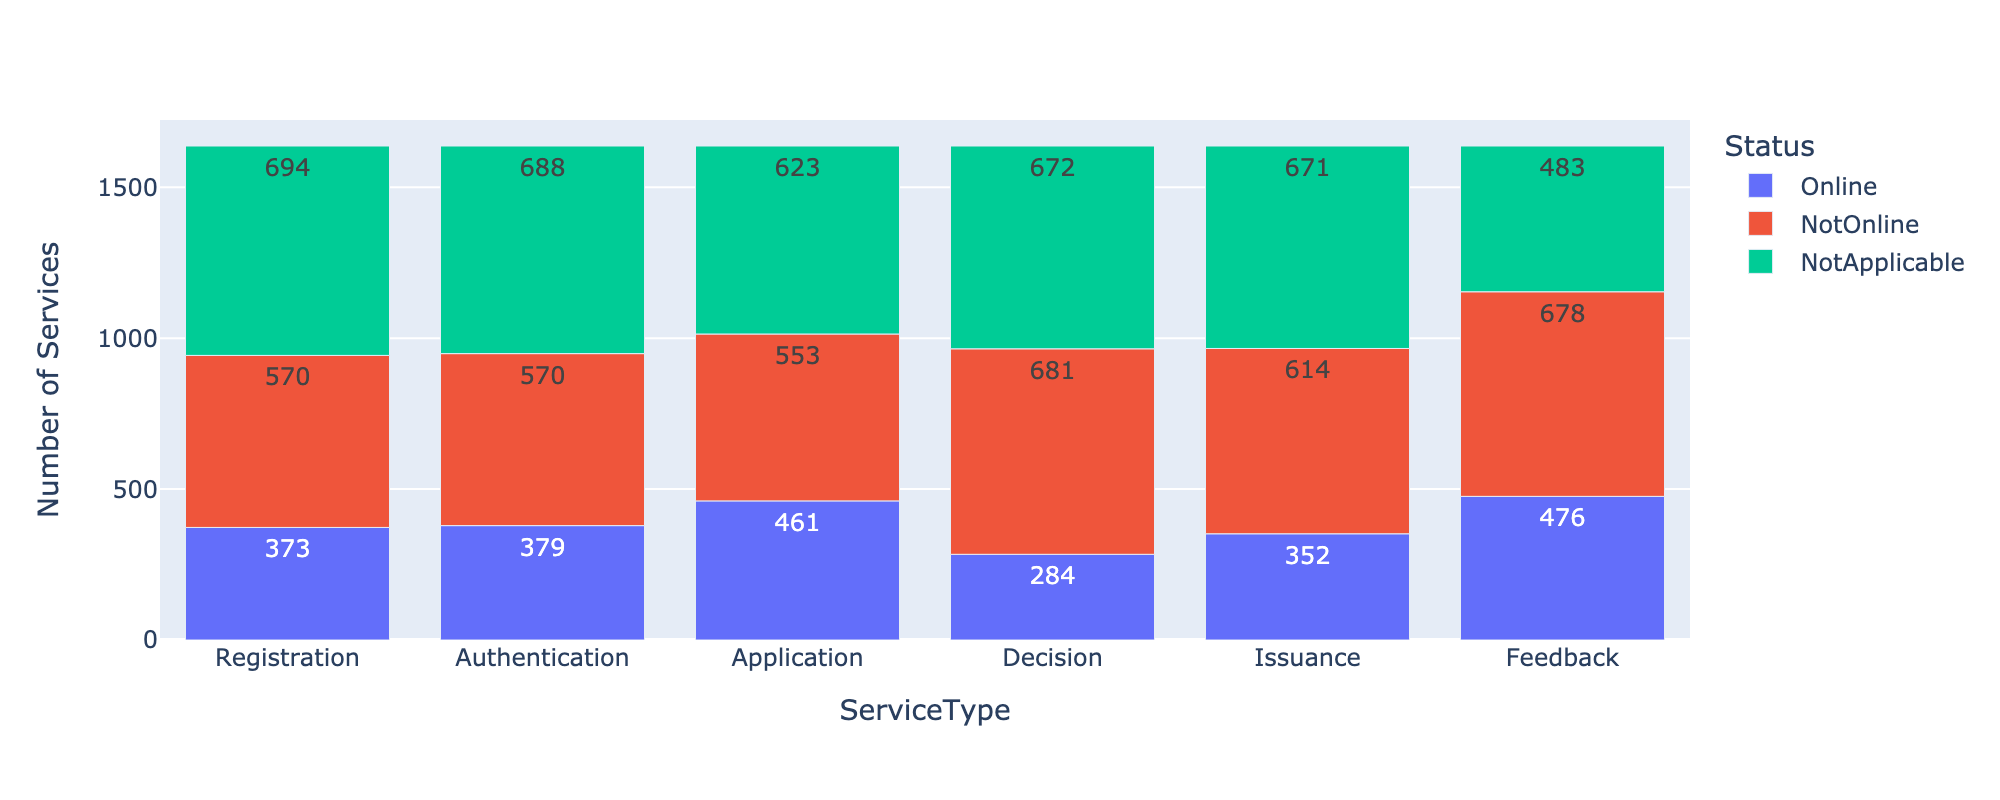
\includegraphics[width=1\linewidth]{OnlineStatus.png}
    \caption{\label{fig:OnlStat}Online Status of Services 2022-2023}
\end{figure}
    